\documentclass[tikz,border=3pt]{standalone}
\usepackage{pgfplots}\pgfplotsset{compat=1.18}
\usetikzlibrary{arrows.meta,positioning,calc}
\begin{document}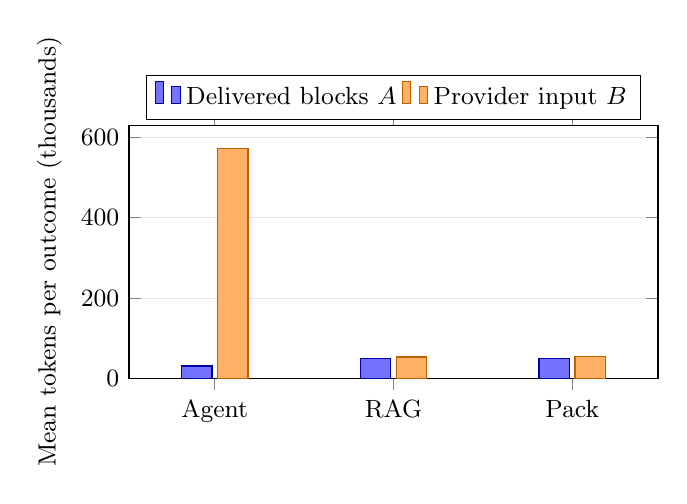
\begin{tikzpicture}
\begin{axis}[width=8.3cm,height=4.8cm,ybar,bar width=11pt,
      symbolic x coords={Agent,RAG,Pack},xtick=data,ymin=0,
      ylabel={Mean tokens per outcome (thousands)},
      tick label style={font=\small},label style={font=\small},
      ymajorgrids=true,grid style={gray!20},
      legend style={at={(.5,1.02)},anchor=south,legend columns=2,font=\small},
      enlarge x limits=.24]
      \addplot[fill=blue!55,draw=blue!65!black] coordinates {(Agent,31.37577500) (RAG,49.99606250) (Pack,49.99435000)};\addlegendentry{Delivered blocks $A$}\addplot[fill=orange!60,draw=orange!75!black] coordinates {(Agent,572.74845833) (RAG,53.63708750) (Pack,54.19368750)};\addlegendentry{Provider input $B$}\end{axis}
\end{tikzpicture}\end{document}
